% a-project.tex, v-1.0.3 marcoreis baseado no
% abntex2-modelo-trabalho-academico.tex, v-1.9.7 laurocesar
% Copyright 2012-2018 by abnTeX2 group at http://www.abntex.net.br/ 
% 
% This work consists of the files ........
% 
% -----------------------------------------------------------------------------
% Modelo para desenvolvimento de documentação de projetos acadêmicos
% (tese de doutorado, dissertação de mestrado e trabalhos de monografias em geral) 
% em conformidade com ABNT NBR 14724:2011: Informação e documentação. 
% -----------------------------------------------------------------------------
% Opções para a documentação
%
% Fancy page headings 
%\documentclass[fancyheadings, subook]{Classes/a-prj}
%\documentclass[fancyheadings, sureport]{Classes/a-prj}
%
% Fancy chapters and sections headings 
%\documentclass[fancychapter, subook]{Classes/a-prj}
%\documentclass[fancychapter, sureport]{Classes/a-prj}
%
% Fancy page , chapters and sections headings
%\documentclass[fancyheadings, fancychapter, subook]{Classes/a-prj}
\documentclass[fancyheadings, fancychapter, sureport]{Classes/a-report}
%
% -----------------------------------------------------------------------------
% Alguns comandos para a fancy page headings)
%
% Page header line width
%\footlinewidth{value}
%
% Page footer line width
%\headlinewidth{value}
%
% Page header and footer line width
%\headingslinewidth{value}
%
% Page header and footer lines without text
%\headingslinesonly
%
% The default line width is 0.3pt.
% Set the value to 0pt to remove the page header and/or footer line
%
% -------------------------------------------------------------------------------
% Formato de figuras suportado
% -------------------------------------------------------------------------------
% O formato das figuras depende da forma como o arquivo de saída é gerado.
% As figuras inseridas na pasta Figures serão automaticamente reconhecidas sem
% a necessidade de inserir a extensão do arquivo.
%
% O pdfLaTEX (PDF) suporta figuras com as extensões: pdf, jpg, png e mps.
%
% -------------------------------------------------------------------------------
% Árvore do diretório a-project.tex
%  Diretório
%       \Classes        (requerido)
%       \Figures        (requerido) --------------------------------->
%       \Figures\PDF    (optional)
%       \Figures\JPG    (optional) Figures located within these
%       \Figures\PNG    (optional) folders are searched automatically
%       \Figures\MPS    (optional)  by the a-prj class.
%       \Figures\EPS    (optional)
%       \Figures\PS     (optional) <--------------------------------
%       \Tables         (requerido)
%       \Others         (requerido)
%       \Chapters       (requerido)
%       \Appendices     (optional)
%       \References     (requerido)
%
% -------------------------------------------------------------------------------
% PDF File resumo
\ifpdf
    \hypersetup{
    	backref,
        colorlinks  = true,
        pdftitle    = Modelo de documentação,
        pdfauthor   = {Marco Reis, marco.a.reis@gmail.com},
        pdfsubject  = Mestre em Engenharia,
        pdfcreator  = Subtitulo,
        pdfproducer = PDFLatex,
        pdfkeywords = {documentação, latex, dissertação, tese}}
 \fi
%
% -------------------------------------------------------------------------------
% Relação de pacotes opcionais utilizados
\usepackage[utf8]{inputenc}
\usepackage[brazil]{babel}
\usepackage{longtable}
\usepackage{dcolumn}
\usepackage{multirow}
\usepackage{lscape}
%\usepackage{graphicx}
\usepackage{rotating}
%\usepackage{float,subfigure}
%\usepackage{graphicx, subfigure}
\usepackage{cite}
\usepackage[left=3cm,top=3cm,right=2cm,bottom=2cm]{geometry}
\usepackage[alf]{abntex2cite}
\usepackage{ifpdf}
\usepackage{shadow}
\usepackage{wrapfig}
\usepackage[normalem]{ulem}
\usepackage{makeidx}
\usepackage{yfonts}
\usepackage{algorithm}
\usepackage{algorithmic}
\usepackage{lmodern}
\usepackage[T1]{fontenc}
\usepackage{indentfirst}
\usepackage{color}
\usepackage{microtype}
\usepackage{lipsum}
\usepackage{caption}
\usepackage{subcaption}
\usepackage{plantuml}
\makeindex 
\setlength{\LTcapwidth}{\textwidth}
%
\newtheorem{theorem}{Teorema}
\newtheorem{definition}[theorem]{Definição}
%
% -------------------------------------------------------------------------------
% Configurações do pacote backref
\renewcommand{\backrefpagesname}{Citado na(s) página(s):~}
% Texto padrão antes do número das páginas
\renewcommand{\backref}{}
% Define os textos da citação
\renewcommand*{\backrefalt}[4]{
	\ifcase #1 %
		Nenhuma citação no texto.%
	\or
		Citado na página #2.%
	\else
		Citado #1 vezes nas páginas #2.%
	\fi
}
% 
% -------------------------------------------------------------------------------
% Início do documento raiz
\begin{document}
% Definição do título da página
    \university{Universidade Positivo}
	%\faculty{Programa de...}
	%\school{Escola de...}
% 
    %\course{Engenharia Elétrica}
    \typework{Relatório Final}
% 
	%\course{Mestrado em Modelagem Computacional e Tecnologia Industrial}
	%\typework{Disserta\c{c}\~ao de mestrado}
	%\typework{Exame de Qualificação de Mestrado}
% 
	%\course{Engenharia Elétrica}
	%\typework{Tese de doutorado}
	%\typework{Exame de Qualificação de doutorado}
%
% -------------------------------------------------------------------------------
% Informações gerais
    \thesistitle{Portfólio Jhenifer}
    \hidevolume
    \thesisvolume{Volume 1 of 1}
    \thesisauthor{Carlos Manoel Nogueira Fernandes}
    \thesisauthorr{Eduardo Rodrigues, Christian Von Ryn}
    \thesisauthorrr{Lucas Pereira Hartinger}
    \thesisauthorrrr{Luis Felipe Fogaça, Luiz Antonio Pacheco Cruz}
    \thesisauthorrrrr{Joao Rodrigo de Oliveira}

    \thesisadvisor{Prof. Marco Reis, M.Eng.}
    %\hidecoadvisor
    %\thesiscoadvisor{Marco Reis}
    \thesismonthyear{Junho de 2025}
% 
    \maketitlepage
%
% ----------------------------------------------------------------------------
% Inserir Folha de rosto, Nota de estilo, folha de assinaturas, dedicatoria
    \begin{folharosto}

\begin{center}
\theauthor \\
\theauthorr \\
\theauthorrr \\
\theauthorrrr \\
\theauthorrrrr \\
\end{center}
\ \\
\ \\
\ \\
\ \\
\ \\
\begin{spacing}{2}
   \begin{center}
   {\LARGE {\bf \thetitle}}
   \end{center}
\end{spacing}
\ \\
\ \\
\ \\
\vspace*{85mm}
% \begin{flushright}

%    \begin{list}{}{
%       \setlength{\leftmargin}{7.5cm}
%       \setlength{\rightmargin}{0cm}
%       \setlength{\labelwidth}{0pt}
%       \setlength{\labelsep}{\leftmargin}}

%       \item \thetypework apresentada ao \thefaculty, Curso de \thecourse
%       do \theuniversity, como requisito parcial para a obten\c{c}\~ao do
%       t\'itulo de {\bf \thedegreetitle}.

%       \begin{list}{}{
%       \setlength{\leftmargin}{0cm}
%       \setlength{\rightmargin}{0cm}
%       \setlength{\labelwidth}{0pt}
%       \setlength{\labelsep}{\leftmargin}}

%       \item \'Area de conhecimento: Interdisciplinar

%       \item Orientador: \theadvisor
%       \newline \hspace*{2.1cm}  %{\it \theuniversity}

%       \end{list}
%    \end{list}

% \end{flushright}
\ \\
\ \\
\ \\
\ \\
%\begin{spacing}{1.5}
   \begin{center}
   Curitiba \par
   \theuniversity \par
   2025
   \end{center}
%\end{spacing}

\end{folharosto}

    %\begin{notaestilo}
Esta \thetypeworkthree foi elaborada considerando as normas de
estilo (i.e. est\'eticas e estruturais) propostas aprovadas pelo
colegiado do \thefacultytwo e est\~ao dispon\'iveis em formato
eletr\^onico ({\it download} na P\'agina Web
http:$//$ead.fieb.org.br$/$portal\_faculdades$/$dissertacoes-e-teses-mcti.html
ou solicita\c{c}\~ao via e-mail \`a secretaria do
programa) e em formato impresso somente para consulta. \\

Ressalta-se que o formato proposto considera diversos itens das
normas da Associa\c{c}\~ao Brasileira de Normas T\'ecnicas (ABNT),
entretanto opta-se, em alguns aspectos, seguir um estilo pr\'oprio
elaborado e amadurecido pelos professores do programa de
p\'os-gradua\c{c}\~ao supracitado.

\end{notaestilo}

    %\begin{folhaassinaturas}

%\thispagestyle{empty}

\def\signature#1#2{\parbox[b]{1in}{\smash{#1}\vskip12pt}
\hfill \parbox[t]{3in}{\shortstack{\vrule width 3in height
0.4pt\\\small#2}}}

\def\InstituicaoMembro#1#2{\parbox[b]{1in}{\smash{#1}\vskip12pt}
\hfill \parbox[t]{3in}{\shortstack{\vrule width 3in \\\small#2}}}

\def\signaturepage{%

    \begin{spacing}{1.5}
        \begin{center}
        {\LARGE \theuniversity} \\
        {\large \thefaculty} \\
        {\large \thecourse} \\
        \end{center}
    \end{spacing}

   \vskip 0.25in plus 0.4in minus 0.1in

    \begin{spacing}{1.5}
        \begin{sloppypar}
        A Banca Examinadora, constitu\'ida pelos professores abaixo
        listados, leram e recomendam a aprova\c{c}\~ao [com distin\c{c}\~ao] da
        \thetypeworktwo, intitulada ``\thetitle",
        apresentada no dia (dia) de (m\^es) de (ano), como requisito
        parcial para a obten\c{c}\~ao do t\'itulo de {\bf \thedegreetitle}.\\
        \end{sloppypar}
    \end{spacing}

    \def\sigskip{\vskip0.15in plus 0.2in minus 0.1in}
    \def\beginskip{\vskip0.3875in plus 0.2in minus 0.1in}

    \beginskip
    \signature{Orientador:}{Prof. Dr. \theadvisor} \\
    \InstituicaoMembro{}{\theuniversity} \\

    \sigskip
    \beginskip
    \signature{Membro externo da Banca:}{Prof. Dr. Nome completo} \\
    \InstituicaoMembro{}{Institui\c{c}\~ao do membro da banca} \\

    \sigskip
    \beginskip
    \signature{Membro externo da Banca:}{Prof. Dr. Nome completo} \\
    \InstituicaoMembro{}{Institui\c{c}\~ao do membro da banca} \\

    %\sigskip
    %\beginskip
   % \signature{Membro interno da Banca:}{Prof. Dr. Nome completo} \\
   % \InstituicaoMembro{}{Institui��o do membro da banca} \\

    \vfill
    \newpage
    \setcounter{page}{3}
}
%*********************************************************************


\signaturepage


\end{folhaassinaturas}

    %\include{Others/dedicatoria}
    %\include{Others/agradecimentos}
%
% ----------------------------------------------------------------------------
% Resumo/abstract, sumário e siglas
    \begin{romanpagenumbers}
        \begin{thesisresumo}
Desenvolver um site de portfólio pessoal para a
 estudante Jhenifer, com foco na apresentação
 profissional de suas informações, projetos,
 habilidades e canais de contato, utilizando
 tecnologias web modernas e seguindo princípios
 de usabilidade e responsividade

\ \\

% use de três a cinco palavras-chave

\textbf{Palavras-chave}: portfólio, estudante, projetos, tecnologias, responsividade

\end{thesisresumo}

        \begin{thesisabastract}
Develop a personal portfolio website for student Jhenifer, focusing on the professional presentation of her information, projects, skills and contact channels, using modern web technologies and following usability and responsiveness principles.

\ \\

% use de tr�s a cinco palavras-chave

\textbf{Keywords}: portfolio, student, projects, technologies, responsiveness

\end{thesisabastract}

        % Make list of contents, tables and figures
        \thesiscontents
        
        %Include other required section
        %\begin{thesisabbreviations}
\begin{footnotesize}
\begin{longtable}[l]{p{2cm}l}
  tprax   \dotfill & \thefaculty \\
  WWW       \dotfill &  World Wide Web \\
\end{longtable}
\end{footnotesize}
\end{thesisabbreviations}

        %\begin{thesissymbols}
\begin{footnotesize}
\begin{longtable}[l]{p{2cm}l}
  $\partial$   \dotfill  & Bla bla bla \\
  $\prod$       \dotfill & ble ble ble \\
  $\partial$   \dotfill  & Bla bla bla \\
  $\prod$       \dotfill & ble ble ble \\
  $\partial$   \dotfill  & Bla bla bla \\
  $\prod$       \dotfill & ble ble ble \\
  $\partial$   \dotfill  & Bla bla bla \\
  $\prod$       \dotfill & ble ble ble \\
  $\partial$   \dotfill  & Bla bla bla \\
  $\prod$       \dotfill & ble ble ble \\
  $\partial$   \dotfill  & Bla bla bla \\
  $\prod$       \dotfill & ble ble ble \\
  $\partial$   \dotfill  & Bla bla bla \\
  $\prod$       \dotfill & ble ble ble \\
  $\partial$   \dotfill  & Bla bla bla \\
  $\prod$       \dotfill & ble ble ble \\
  $\partial$   \dotfill  & Bla bla bla \\
  $\prod$       \dotfill & ble ble ble \\
  $\partial$   \dotfill  & Bla bla bla \\
  $\prod$       \dotfill & ble ble ble \\
  $\partial$   \dotfill  & Bla bla bla \\
  $\prod$       \dotfill & ble ble ble \\
  $\partial$   \dotfill  & Bla bla bla \\
  $\prod$       \dotfill & ble ble ble \\
  $\partial$   \dotfill  & Bla bla bla \\
  $\prod$       \dotfill & ble ble ble \\
  $\partial$   \dotfill  & Bla bla bla \\
  $\prod$       \dotfill & ble ble ble \\
  $\partial$   \dotfill  & Bla bla bla \\
  $\prod$       \dotfill & ble ble ble \\
  $\partial$   \dotfill  & Bla bla bla \\
  $\prod$       \dotfill & ble ble ble \\
  $\partial$   \dotfill  & Bla bla bla \\
  $\prod$       \dotfill & ble ble ble \\
  $\partial$   \dotfill  & Bla bla bla \\
  $\prod$       \dotfill & ble ble ble \\
  $\partial$   \dotfill  & Bla bla bla \\
  $\prod$       \dotfill & ble ble ble \\          
\end{longtable}
\end{footnotesize}
\end{thesissymbols}

        %Switch the page numbering back to the default format
    \end{romanpagenumbers}
%
% ---------------------------------------------------------------------------
% Include thesis chapters
    \parskip=\baselineskip
    \chapter{Introdução}
\label{chap:intro}

% Este pode ser um parágrafo citado por alguém \cite{Barabasi2003-1} e \cite{barabasi2003linked}.
% Para ajustar veja o comentário do capítulo \ref{chap:fundteor}.

% As orientações do robô \cite{aperea-1}.

% fakdfjlsdjfldsjfldsj
% dfkhfdskfhkdjh


% Segundo \citeonline{barabasi2003linked}, ...

% 
% \loremipsum dolor sit amet, consectetur adipiscing elit. Sed do eiusmod tempor incididunt ut labore et dolore magna aliqua. Ut enim ad minim veniam, quis nostrud exercitation ullamco laboris nisi ut aliquip ex ea commodo consequat. Duis aute irure dolor in reprehenderit in voluptate velit esse cillum dolore eu fugiat nulla pariatur. Excepteur sint occaecat cupidatat non proident, sunt in culpa qui officia deserunt mollit anim id est laborum.
%--------- NEW SECTION ----------------------
\section{Objetivos}

\label{sec:obj}

\label{sec:obj}

\subsection{Objetivos Específicos}
\label{ssec:objesp}

O projeto tem como principal objetivo o desenvolvimento de um portfólio pessoal profissional para o cliente, com foco em:
\begin{itemize}
      \item Apresentar informações pessoais e profissionais de forma clara e atrativa;
      \item Reunir informações relevantes, como experiências, habilidades técnicas, formação e projetos desenvolvidos;
      \item Facilitar o contato com recrutadores e empresas, por meio de um formulário funcional e links para redes sociais;
      \item Aumentar a presença online do cliente, com um site responsivo acessível em diferentes dispositivos;
      \item Proporcionar autonomia, permitindo futuras atualizações de conteúdo de maneira simples;
      \item Utilizar boas práticas de desenvolvimento, garantindo desempenho, acessibilidade e escalabilidade;
\end{itemize}

\subsubsection*{Objetivos específicos principais}
\label{sssec:obj-principais}



%--------- NEW SECTION ----------------------
\section{Justificativa}
\label{sec:justi}

O desenvolvimento de um portfólio pessoal se justifica por diversos fatores estratégicos e profissionais. Abaixo, estão os principais motivos que fundamentam este projeto 
\begin{itemize}
\item Fortalecimento da presença digital
\item Centralização de informações
\item Valorização da imagem profissional
\item Autonomia e flexibilidade
\item Aprendizado e desenvolvimento técnico
\end{itemize}
%--------- NEW SECTION ----------------------
\section{Organização do documento}
\label{section:organizacao}

Este documento apresenta $5$ capítulos e está estruturado da seguinte forma:

\begin{itemize}

  \item \textbf{Capítulo \ref{chap:intro} - Introdução}: Contextualiza o âmbito, no qual a pesquisa proposta está inserida. Apresenta, portanto, a definição do problema, objetivos e justificativas da pesquisa e como este \thetypeworkthree está estruturado;
  \item \textbf{Capítulo \ref{chap:fundteor} - Fundamentação Teórica}: * Fundamentação Teórica: Apresenta os principais conceitos relacio-nados ao desenvolvimento web, design responsivo, usabilidade, metodologias ágeis eferramentas utilizadas no projeto;
  \item \textbf{Capítulo \ref{chap:metod} - Materiais e Métodos}: * Materiais e Métodos: Descreve a metodologia adotada (modeloWaterfall), os processos de levantamento de requisitos, prototipação, implementação,além das ferramentas utilizadas durante o desenvolvimento;
  \item \textbf{Capítulo \ref{chap:result} - Resultados}: * Resultados: Apresenta o produto final desenvolvido, as funcionali-dades implementadas, os testes realizados, o feedback do cliente e a validação doprojeto;
  \item \textbf{Capítulo \ref{chap:conc} - Conclusão}: Apresenta as conclusões, contribuições e algumas sugestões de atividades de pesquisa a serem desenvolvidas no futuro.

\end{itemize}

    \chapter{Conceito do projeto do portfólio}
\label{chap:fundteor}
%--------- NEW SECTION ----------------------

% isso é igual <=  === <> #{ #( www
% <| |>
% ===

Lista dos documentos
\begin{enumerate}
   \item diagrama de classe
   \item diagrama de casos de uso
   \item diagrama de sequência
\end{enumerate}


Neste capítulo serão abordados os requisitos do cliente, os requisistos técnicos e a pesquisa por similares. 



%conferir se precisa de requisitos do cliente
\section{Requisitos do cliente}
 O cliente definiu certos requisitos quanto à operação e  às características do portfólio:
 \begin{itemize}
    \item Portfólio simples;
    \item Informações de contato;
    \item Mensagem automática para o e-mail da cliente;
    \item Mostrar as tecnologias e linguagens que domina;
    \item Detalhes em cor de Rosa;
 \end{itemize}

 \section{Requisitos funcionais}
 
 \begin{itemize}
 \item RF001 - Exibir informações pessoaisApresentar nome, formação acadêmica, contatos (email, telefone,etc.) e umabreve descrição sobre o estudante;
 \item RF002 - Listar projetos desenvolvidosListar projetos com informações como título, descrição,tecnologias usadas elinks para repositórios (como GitHub) ou demos;
 \item RF003 - Exibir habilidades técnicasListar linguagens de programação, frameworks, bancos de dados eoutrasferramentas que o estudante domina;
 \item RF004 - Permitir contatoFormulário de contato (ou redirecionar paraemail/mensagem) para que visitantespossam enviar mensagens;
 \item RF005 - Responsividade;
 \item RF006 - Integração com redes sociais Botões/links para GitHub, LinkedIn, Instagram;
\end{itemize}



%  \section{Missão}
%  \lipsum
%  %desenvolver mais
%  Além disso, o Walker deve realizar um desafio, que consiste em navegar de forma autônoma, se localizar por meio de tags e encontrar um determinado objeto.



%  \section{Pesquisa por similares}


% %----------------------------------------------------------

% %--------- NEW SECTION ----------------------


% %---------------picture------------------------------------
% % \begin{figure}
% %     \centering
% %     \subfigure[Figure A]{\label{fig:a}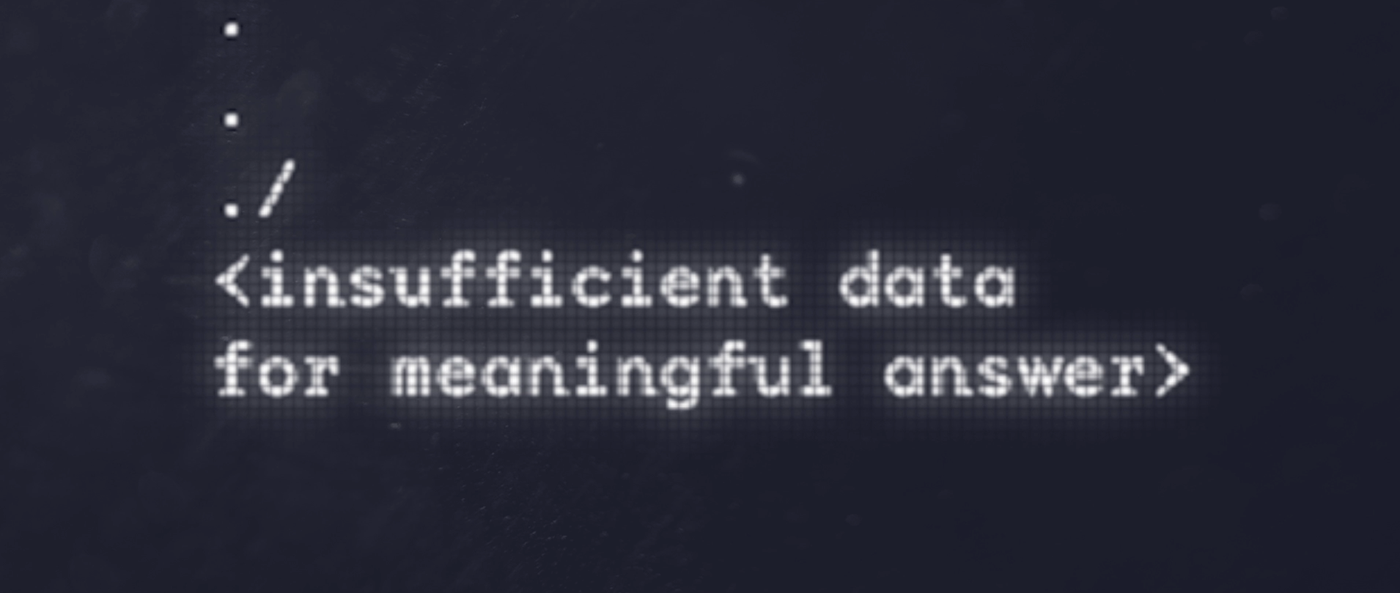
\includegraphics[width=60mm]{./lq}}
% %     \subfigure[Figure B]{\label{fig:b}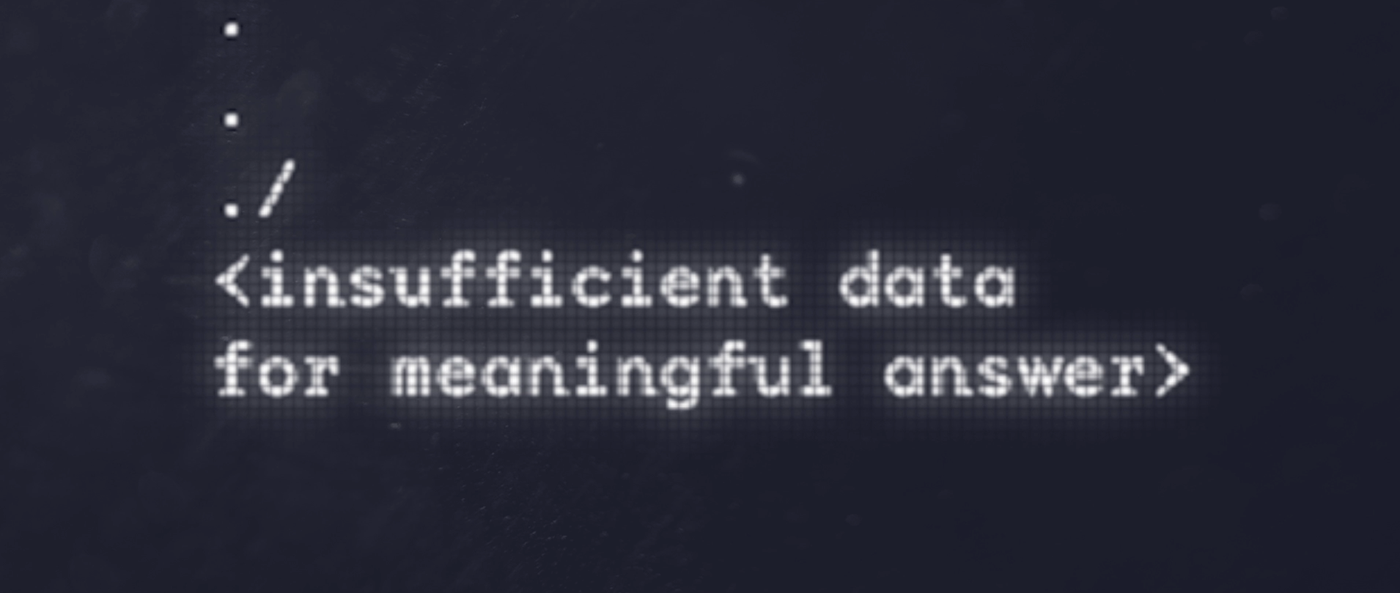
\includegraphics[width=60mm]{./lq}}
% %     \subfigure[Figure C]{\label{fig:c}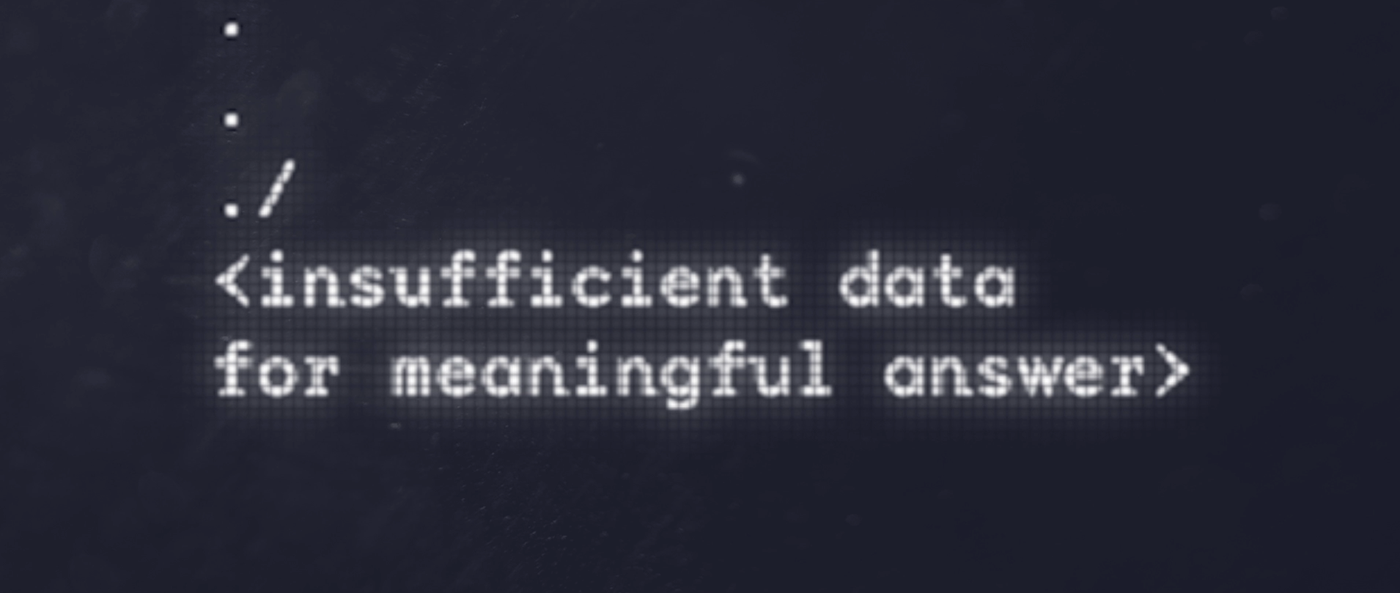
\includegraphics[width=\textwidth]{./lq}}
% %     \caption{Three simple graphs}
% %     \label{fig:three graphs}
% % \end{figure}
% %----------------------------------------------------------

% % \begin{figure}
% %     \centering
% %     \begin{subfigure}[b]{0.3\textwidth}
% %         \centering
% %         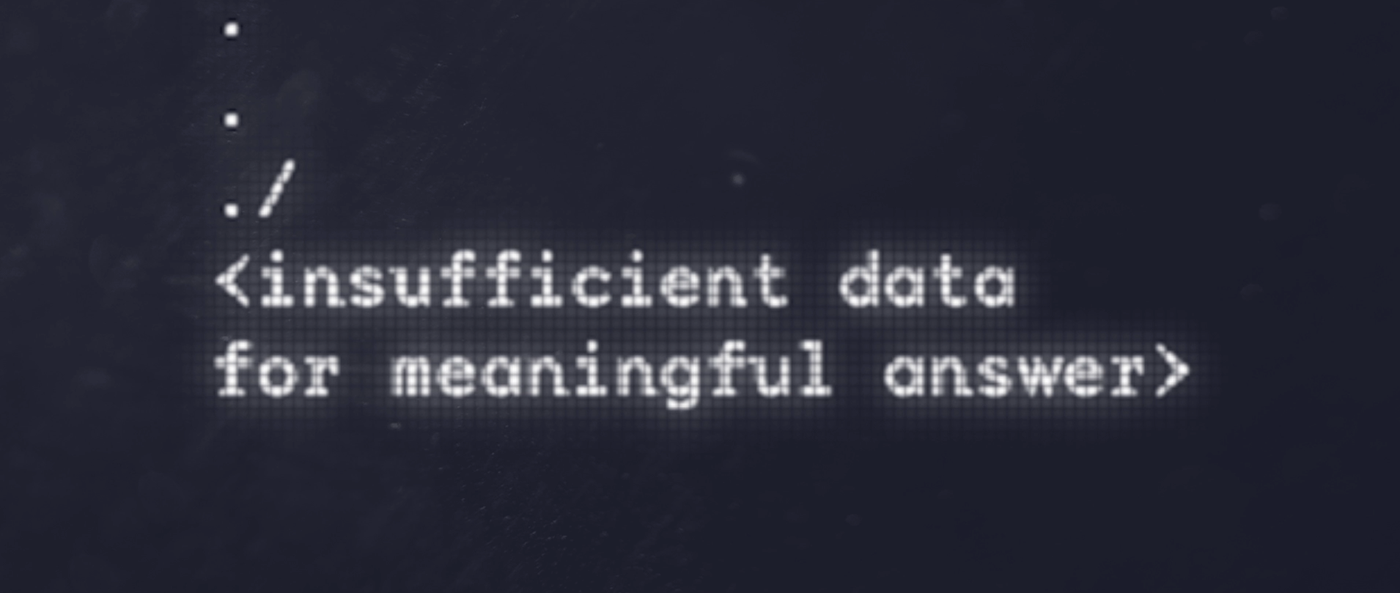
\includegraphics[width=\textwidth]{./lq}
% %         \caption{$y=x$}
% %         \label{fig:y equals x}
% %     \end{subfigure}
% %     \hfill
% %     \begin{subfigure}[b]{0.3\textwidth}
% %         \centering
% %         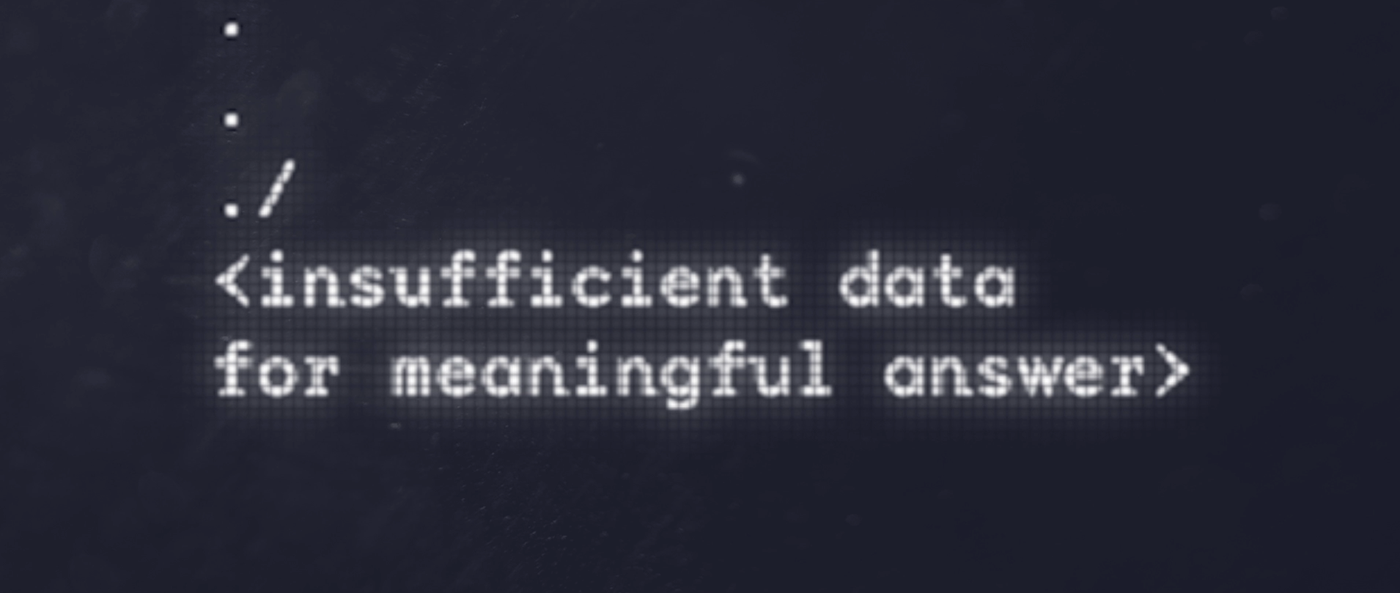
\includegraphics[width=\textwidth]{./lq}
% %         \caption{$y=3sinx$}
% %         \label{fig:three sin x}
% %     \end{subfigure}
% %     \hfill
% %     \begin{subfigure}[b]{0.3\textwidth}
% %         \centering
% %         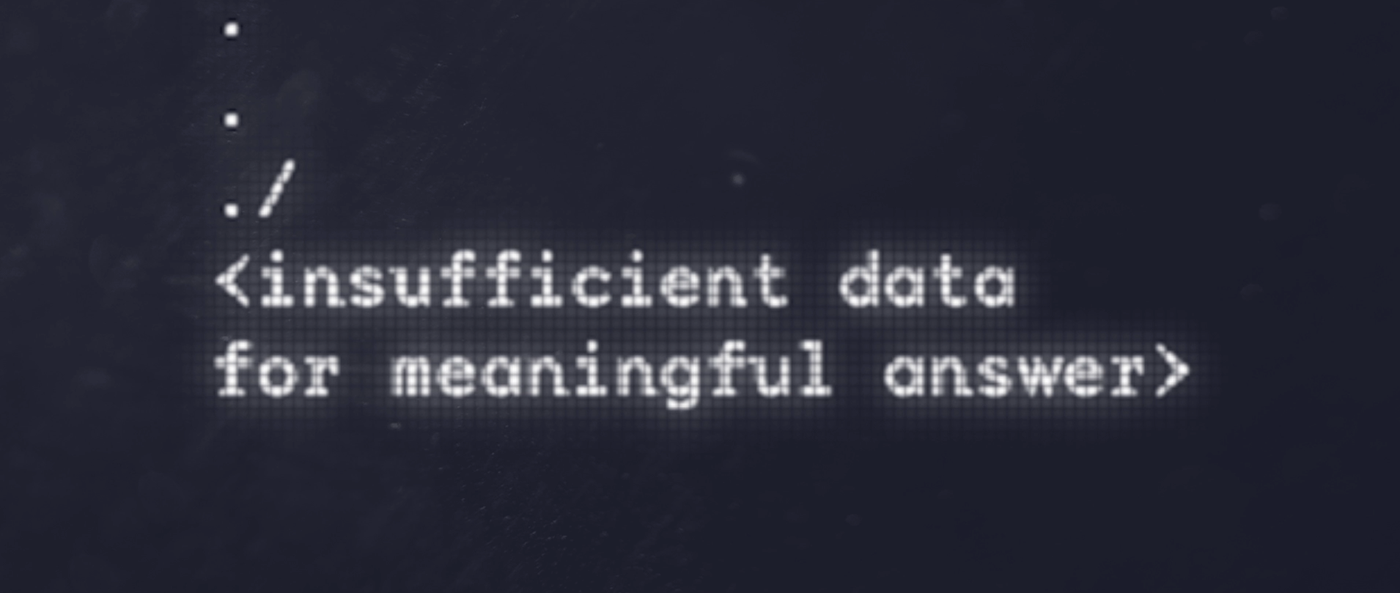
\includegraphics[width=\textwidth]{./lq}
% %         \caption{$y=5/x$}
% %         \label{fig:five over x}
% %     \end{subfigure}
% %        \caption{Three simple graphs}
% %        \label{fig:three graphs}
% % \end{figure}


% % %--------- NEW SECTION ----------------------
% % \section{Assunto 2}
% % \label{sec:ass2}
% % flkjasdlkfjasdlkfjs

% % \begin{table}[h]
% %     \begin{subtable}[h]{0.45\textwidth}
% %         \centering
% %         \begin{tabular}{l | l | l}
% %         Day & Max Temp & Min Temp \\
% %         \hline \hline
% %         Mon & 20 & 13\\
% %         Tue & 22 & 14\\
% %         Wed & 23 & 12\\
% %         Thurs & 25 & 13\\
% %         Fri & 18 & 7\\
% %         Sat & 15 & 13\\
% %         Sun & 20 & 13
% %        \end{tabular}
% %        \caption{First Week}
% %        \label{tab:week1}
% %     \end{subtable}
% %     \hfill
% %     \begin{subtable}[h]{0.45\textwidth}
% %         \centering
% %         \begin{tabular}{l | l | l}
% %         Day & Max Temp & Min Temp \\
% %         \hline \hline
% %         Mon & 17 & 11\\
% %         Tue & 16 & 10\\
% %         Wed & 14 & 8\\
% %         Thurs & 12 & 5\\
% %         Fri & 15 & 7\\
% %         Sat & 16 & 12\\
% %         Sun & 15 & 9
% %         \end{tabular}
% %         \caption{Second Week}
% %         \label{tab:week2}
% %      \end{subtable}
% %      \caption{Max and min temps recorded in the first two weeks of July}
% %      \label{tab:temps}
% % \end{table}
    \chapter{Desenvolvimento do projeto}
\label{chap:metod}
Nesta seção será descrito o procedimento utilizado para construção inicial do portfólio, incluindo as fases conceitual e design.  Será apresentado a ideação do projeto, especificações e as funcionalidades.

\subsection{Metodologia do projeto}
A metodologia adotada para o desenvolvimento do portfólio do cliente seguiu um processo estruturado em etapas, com foco na personalização, usabilidade e alinhamento com os objetivos profissionais do cliente. As fases principais do projeto foram:

1. Levantamento de Requisitos
Inicialmente, foi realizada uma reunião com o cliente para compreender seus objetivos, público-alvo, preferências visuais e conteúdos a serem incluídos no portfólio. Foram levantadas informações como áreas de atuação, projetos realizados, formação, habilidades e experiências profissionais. Esse levantamento guiou toda a concepção do projeto.

2. Planejamento e Estruturação
Com base nos requisitos, foi definida a estrutura do site (mapa de navegação), os principais blocos de conteúdo (sobre, projetos, habilidades, contato etc.) e os recursos funcionais desejados (como formulário de contato, integração com redes sociais ou repositórios de código). Também foram definidas as tecnologias a serem utilizadas no desenvolvimento.

3. Criação do Design
Foi desenvolvido um layout responsivo e personalizado, baseado nas referências visuais fornecidas pelo cliente e nas boas práticas de design. O protótipo foi validado com o cliente antes do início do desenvolvimento para garantir alinhamento com suas expectativas.

4. Desenvolvimento
O desenvolvimento foi feito utilizando tecnologias web modernas. O código foi estruturado visando desempenho, acessibilidade e facilidade de manutenção. Todo o conteúdo foi inserido de forma dinâmica e otimizada para diferentes dispositivos.

5. Testes e Ajustes
Após a finalização do desenvolvimento, foram realizados testes funcionais, de responsividade e compatibilidade com diferentes navegadores e dispositivos. Ajustes finos foram feitos com base no feedback do cliente.
\section{Ideação}
%escrever oq sera apresentado

\subsection{Arquitetura Geral}
Arquitetura do Projeto
A arquitetura do projeto foi planejada para garantir modularidade, escalabilidade, desempenho e facilidade de manutenção. A estrutura contempla tanto os aspectos técnicos quanto organizacionais do sistema, com foco na entrega de um portfólio moderno, responsivo e funcional.
\begin{itemize}


\item 1. Arquitetura de CamadasO projeto foi dividido em camadas lógicas para organizar melhor as responsabilidades:
\item 2. Camada de Apresentação (Front-end):Responsável pela interface do usuário e experiência de navegação. Desenvolvida com tecnologias web como HTML5, CSS3. Esta camada consome os dados estruturados (projetos, informações pessoais etc.) e os exibe de forma dinâmica.
\item 3. Camada de Dados (Content Layer):Os dados do portfólio ou integrados a um CMS leve para permitir atualizações sem editar código.
\item 4. Camada de Publicação/Servidor (Back-end e Hosting):Em projetos estáticos, esta camada pode ser composta apenas por um serviço de hospedagem como GitHub Pages. 

A arquitetura contempla o uso de design responsivo com media queries e classes utilitárias, garantindo compatibilidade com dispositivos móveis, tablets e desktops. Padrões de acessibilidade como contraste de cores, semântica HTML e navegação por teclado também foram considerados.

\end{itemize}

 	



%desdobramento da função qualidade
% \subsection{Quality Function Deployment}
% \textit{Quality Function Deployment} é uma ferramenta de qualidade que auxilia na conversão das demandas do cliente em características de qualidade do produto. Dessa forma, no primeiro ciclo do QFD foram analisados os requisistos do cliente e os requisitos técnicos necessários, sinalizando os pontos mais importantes e as relações entre estes. O resultado foi exposto na \ref{fig:QFD}

% \begin{figure} [h!]	
%     \centering
%     \caption{ Primeiro ciclo QFD}
%     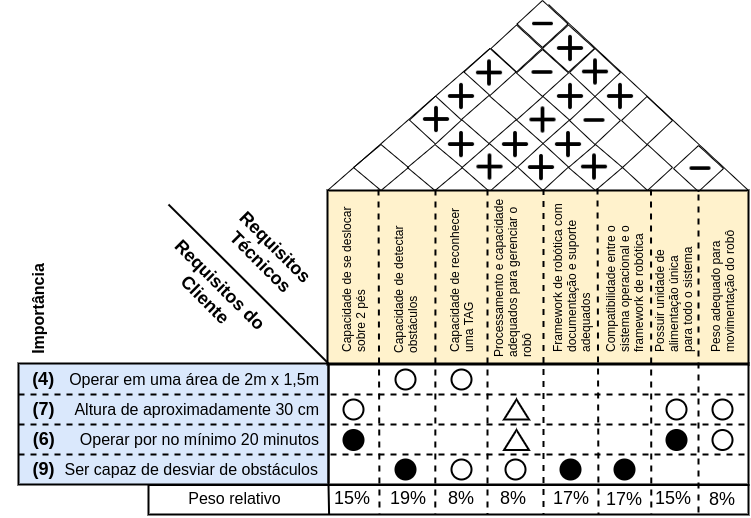
\includegraphics[width=0.8\textwidth]{Figures/QFD}
%     \caption*{Fonte: Autoria própria.}
%     \label{fig:QFD}
% \end{figure}
%  Através do QFD foi possível observar 

% % %--------- NEW SECTION ----------------------
% % \section{Interface do Usuário}
% % \label{sec:ui}
% % \lipsum[1]

% % %--------- NEW SECTION ----------------------
% % \section{Simulação do sistema}
% % \label{sec:sim}
% % \lipsum[2-4]
\subsection{Modelagem dos processos}

\begin{figure} [h!]	
    \centering

    \caption{Modelo esquemático dos processos}
    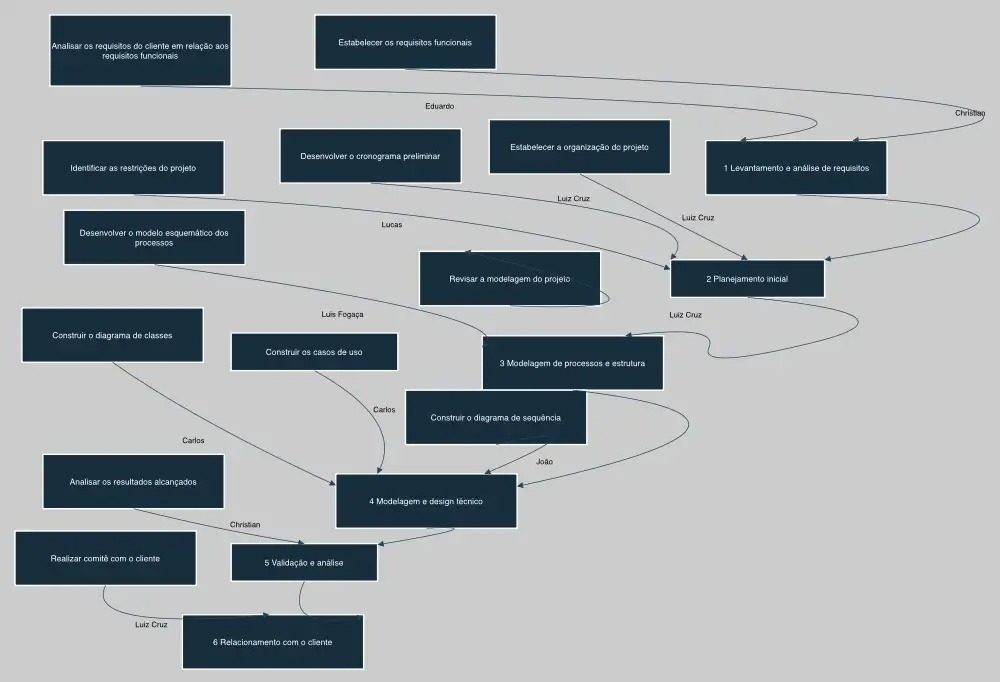
\includegraphics[width=0.9\textwidth]{Figures/Modelagem-dos-processos.jpg}
    \caption*{Fonte: Autoria própria.}
    \label{fig:Modelagem-dos-processos}
\end{figure}
    \chapter{Resultados}
\label{chap:result}
O principal objetivo deste projeto foi adaptar o site do portfólio às expectativas e
 necessidades da Jhenifer. Durante essa jornada, conseguimos avançar de forma
 consistente, completando todas as etapas previstas para o GATE A. Isso incluiu um
 levantamento detalhado dos requisitos junto à cliente, definição da estrutura
 organizacional, criação do cronograma preliminar e realização de reuniões e workshops
 essenciais para garantir que tudo estivesse bem alinhado.
 No GATE B, continuamos evoluindo e validando as principais peças de modelagem do
 sistema, como o diagrama de sequência e o diagrama de classes. Além disso, realizamos
 um comitê com a cliente, o que foi fundamental para validar parte das entregas e garantir
 que o projeto estivesse indo na direção certa.
 Em resumo, tudo o que foi feito até agora resultou em um planejamento bem estruturado,
 na criação das modelagens necessárias para aprimorar o site e na validação inicial junto à
 cliente. Com isso, estabelecemos uma base sólida para dar continuidade ao projeto e
 concluí-lo conforme os objetivos planejados.
% %--------- NEW SECTION ----------------------
% \section{Testes unitários}
% \label{sec:testu}
% \lipsum[1]

% \section{Integração do sistema}
% \label{sec:intsis}
% \lipsum[1]

% %--------- NEW SECTION ----------------------
% \section{Testes integrados}
% \label{sec:testi}
% \lipsum[1]

\section{Diagrama de classes}
\label{sec:class}
O diagrama de classes é uma representação visual das classes do sistema e seus relacionamentos. Ele é utilizado para descrever a estrutura do sistema e como as classes interagem entre si. A Figura \ref{fig:Diagrama_de_classes} apresenta o diagrama de classes do sistema desenvolvido.
\begin{figure} [h!]	
    \centering
    \caption{Meu diagrama de classes}
    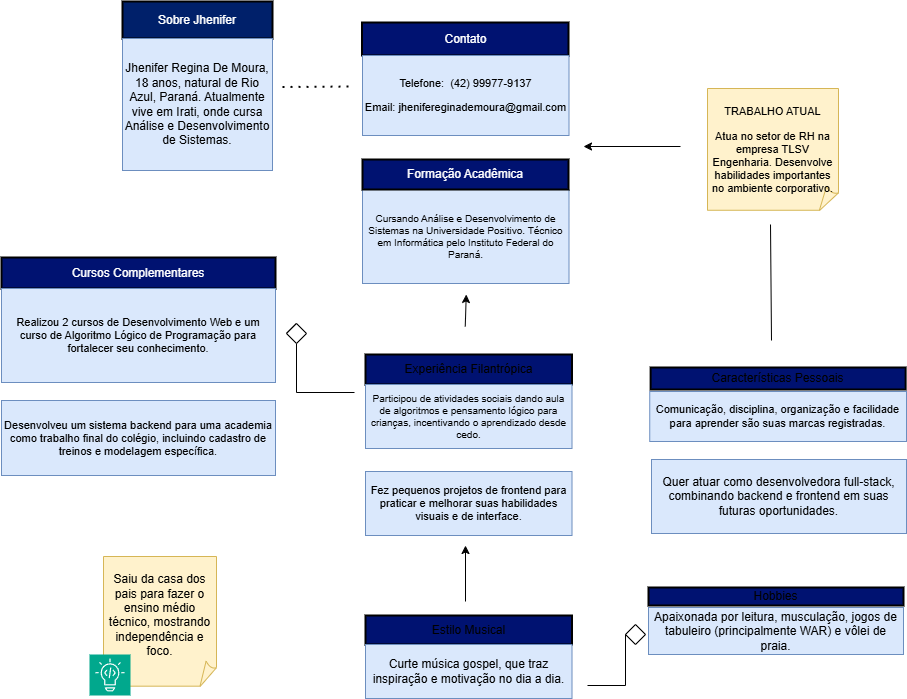
\includegraphics[width=0.8\textwidth]{Figures/Diagrama_de_Classes.png}
    \caption*{Fonte: Autoria própria.}
    \label{fig:Diagrama_de_classes}
\end{figure}

favor olhar a seção \ref{sec:class}.


\section{Diagrama de casos de uso}
\label{sec:casos}
O diagrama de casos de uso é uma representação visual dos casos de uso do sistema e os atores envolvidos. Ele é utilizado para descrever as funcionalidades do sistema e como os usuários interagem com ele. A Figura \ref{fig:casos_de_uso} apresenta o diagrama de casos de uso do sistema desenvolvido.
\begin{figure} [h!] 
    \centering
    \caption{Meu diagrama de casos de uso}
    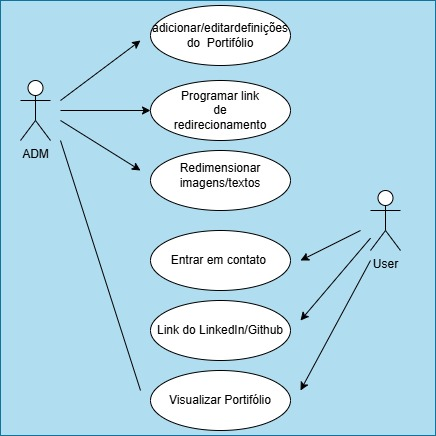
\includegraphics[width=0.8\textwidth]{Figures/casos_de_uso.jpg}
    \caption*{Fonte: Autoria própria.}
    \label{fig:casos_de_uso}
\end{figure}

favor olhar a seção \ref{sec:casos}.

\section{Diagrama de sequência}
\label{sec:sequencia}   
O diagrama de sequência é uma representação visual da interação entre os objetos do sistema ao longo do tempo. Ele é utilizado para descrever como os objetos interagem entre si para realizar uma determinada funcionalidade. A Figura \ref{fig:Diagrama_de_sequencia} apresenta o diagrama de sequência do sistema desenvolvido. 
\begin{figure} [h!] 
    \centering
    \caption{Meu diagrama de sequência}
    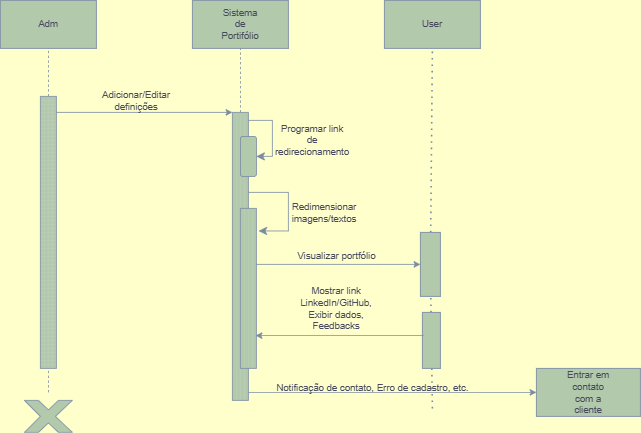
\includegraphics[width=0.8\textwidth]{Figures/Diagrama_de_sequencia.png}
    \caption*{Fonte: Autoria própria.}
    \label{fig:Diagrama_de_sequencia}
\end{figure}

favor olhar a seção \ref{sec:sequencia}.




    \chapter{Conclusão}
\label{chap:conc}

O desenvolvimento do portfólio pessoal para o cliente foi concluído com êxito, atendendo aos requisitos propostos desde a fase inicial de levantamento até a entrega final. O resultado é uma aplicação web moderna, responsiva e de fácil navegação, que cumpre sua principal função: apresentar de forma clara, profissional e atrativa as informações, habilidades e projetos do cliente.

Durante o processo, foi possível aplicar boas práticas de design e desenvolvimento, garantindo uma experiência do usuário agradável, compatibilidade com diferentes dispositivos e navegadores, além de permitir ao cliente futuras atualizações com facilidade. O portfólio também oferece recursos importantes como formulário de contato funcional, integração com redes sociais e estrutura escalável.

A entrega final representa não apenas uma ferramenta de divulgação profissional para o cliente, mas também um produto digital com qualidade técnica e estética. O projeto contribuiu para o fortalecimento da presença online do cliente e está preparado para evoluir conforme suas necessidades cresçam.


\section{Considerações finais}
\label{sec:consid}

Este projeto representou uma oportunidade valiosa de aplicar conhecimentos técnicos em um contexto real, com foco na entrega de um produto funcional, esteticamente agradável e alinhado às necessidades do cliente. O portfólio desenvolvido cumpre seu papel como ferramenta de apresentação profissional e está pronto para ser expandido ou adaptado conforme futuras demandas.

    % include more chapters ...
%
% ----------------------------------------------------------------------------
% Include thesis appendices
    \begin{thesisappendices}
        % Thesis Appendix -------------------------------------------------------



        % Thesis Appendix -------------------------------------------------------




        %% Thesis Appendix -------------------------------------------------------

\chapter{Logbook}
\label{Append:log}



    \end{thesisappendices}
%
% ----------------------------------------------------------------------------
% Configurar as referencias bibliograficas
	\renewcommand\bibname{Referências}
    \addcontentsline{toc}{chapter}{Referências}
    \bibliography{References/referencias}
%
% ----------------------------------------------------------------------------
% Finishing him
    \include{Others/ultimafolha}
\end{document}
%
% -------------------------------------------------------------------------------
% Aqui termina a formatação para o documento.
% In God We Trust. All Other Bring Data. 
%
% -------------------------------------------------------------------------------